\documentclass[a4j]{jarticle}

\usepackage[dvipdfmx]{graphicx}
\usepackage{url}
\usepackage{listings,jlisting}
\usepackage{ascmac}
\usepackage{amsmath,amssymb}

%ここからソースコードの表示に関する設定
\lstset{
  basicstyle={\ttfamily},
  identifierstyle={\small},
  commentstyle={\smallitshape},
  keywordstyle={\small\bfseries},
  ndkeywordstyle={\small},
  stringstyle={\small\ttfamily},
  frame={tb},
  breaklines=true,
  columns=[l]{fullflexible},
  numbers=left,
  xrightmargin=0zw,
  xleftmargin=3zw,
  numberstyle={\scriptsize},
  stepnumber=1,
  numbersep=1zw,
  lineskip=-0.5ex
}
%ここまでソースコードの表示に関する設定

\title{知能プログラミング演習II 課題3}
\author{グループ07\\
  29114086 飛世裕貴\\
%  {\small (グループレポートの場合は、グループ名および全員の学生番号と氏名が必要)}
}
\date{2019年10月28日}

\begin{document}
\maketitle

\paragraph{提出物} rep3
\paragraph{グループ} グループ07
\paragraph{メンバー}
\begin{tabular}{|c|c|c|}
  \hline\hline
  学籍番号&名前&貢献度\\
  \hline\hline
  29114007&池口弘尚&\\
  \hline
  29114031&大原拓人&\\
  \hline
  29114048&北原太一&\\
  \hline
  29114086&飛世裕貴&\\
  \hline
  29114095&野竹浩二朗&\\
  \hline
\end{tabular}



\section{課題の説明}
\begin{description}
\item[課題3-1] セマンティックネットのプログラムを参考に,グループメンバー全員(およびその周辺人物)についてのセマンティックネットを構築せよ.
個人レポートには自分のみ(とその周辺)に関するセマンティックネットを示し,グループレポートには全員(とその周辺)に関するセマンティックネットを示せ

\item[課題3-2] フレームのプログラムを参考に,自分達の興味分野に関する知識をフレームで表現せよ.その分野の知識を表す上で必須となるスロットが何かを考え,クラスフレームを設計すること.
個人レポートには自分が作ったインスタンスフレームのみ(クラスフレームの設計担当者はクラスフレームも)を示し,グループレポートにはクラスフレームおよび全員分のインスタンスフレームを示せ.
\item[課題3-3] 課題3-1または3-2で作った知識表現を用いた質問応答システムを作成せよ.
なお,ユーザの質問は英語や日本語のような自然言語が望ましいが,難しければ課題2で扱ったような変数を含むパターン (クエリー) でも構わない.

\item[課題3-4]課題3-1または3-2で作った知識表現を図として示すためのユーザインターフェース(GUI) を設計し実装せよ。
\item[課題3-5] DBpedia Japaneseは,Wikipedia日本語版から生成された知識表現から成る巨大な知識ベースである.またWikidataは,誰でも直接編集できる知識ベースである。
上記3-3で作成した質問応答システムを,DBpediaあるいはWikidata中の知識を使って質問に答えられるよう,拡張せよ.

\end{description}

今回、私が担当した課題は課題3-1、3-2、3-3である。

\section{課題3-1}
\begin{screen}
 セマンティックネットのプログラムを参考に,グループメンバー全員(およびその周辺人物)についてのセマンティックネットを構築せよ.
個人レポートには自分のみ(とその周辺)に関するセマンティックネットを示し,グループレポートには全員(とその周辺)に関するセマンティックネットを示せ
\end{screen}

\subsection{手法}
ここで構築したセマンティックネットは下図のようなものである.

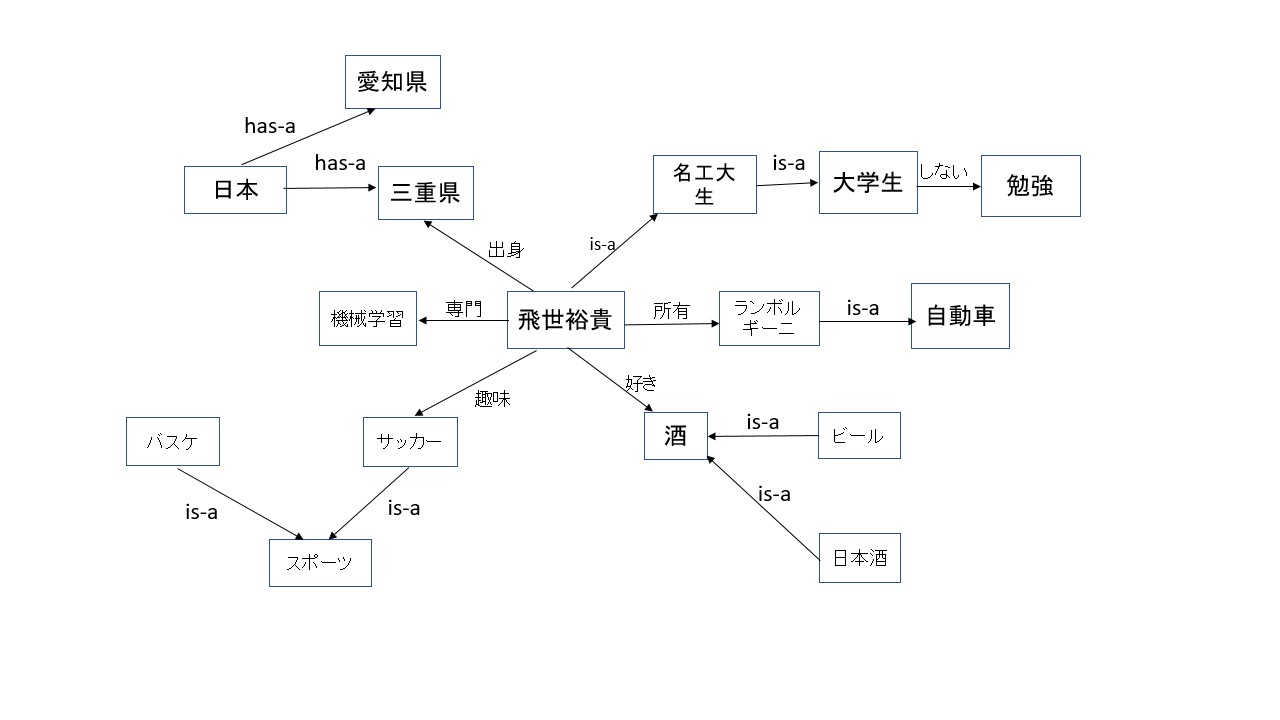
\includegraphics[width=150mm,height=80mm]{Slide2.jpg}

\subsection{実装}
上に示したセマンティックネットをMakeSemanticNet.javaにおいて生成する.セマンティックネットの生成はExample.javaを元に実装した.

\subsection{実行例}
MakeSemanticNet.javaによってセマンティックネットを生成した.その結果を以下に示す.

\begin{screen}
\begin{verbatim}
飛世裕貴  =is-a=>  名工大生
飛世裕貴  =所有=>  ランボルギーニ
飛世裕貴  =好き=>  酒
飛世裕貴  =趣味=>  サッカー
飛世裕貴  =専門=>  機械学習
飛世裕貴  =出身=>  三重県
名工大生  =is-a=>  大学生
( 飛世裕貴  =is-a=>  大学生 )
大学生  =しない=>  勉強
( 名工大生  =しない=>  勉強 )
( 飛世裕貴  =しない=>  勉強 )
ランボルギーニ  =is-a=>  自動車
ビール  =is-a=>  酒
日本酒  =is-a=>  酒
サッカー  =is-a=>  スポーツ
バスケ  =is-a=>  スポーツ
日本  =has-a=>  三重県
日本  =has-a=>  愛知県
\end{verbatim}
\end{screen}

このように図に示したものと同様のセマンティックネットが生成されたことを確認した.

\subsection{考察}
今回生成したセマンティックネットはデータ同士の関係を記述する上で、有用なものであると考える.プログラミング言語において、データ同士の構造的関連を記述する機能は存在するが、セマンティックネットにおいては構造的な繋がりのみでなく意味的な繋がりについても記述することができる.例えば、Javaにおいてクラスを用いる事でデータの包含関係を記述する事ができるがそのデータ同士が意味的にどのような繋がりがあるか理解するためには人間がコードを見て理解する以外にないだろう.しかし、セマンティックネットにおいてはデータ同士のつながりを表すリンクに構造的関係だけでなく意味的関係を持たせている為、人間にも理解しやすく、また人間が用いる自然言語の意味推論や知識構造を表現する上で効果的なデータ構造と言える.


\section{課題3-2}
\begin{screen}
フレームのプログラムを参考に,自分達の興味分野に関する知識をフレームで表現せよ.その分野の知識を表す上で必須となるスロットが何かを考え,クラスフレームを設計すること.
個人レポートには自分が作ったインスタンスフレームのみ(クラスフレームの設計担当者はクラスフレームも)を示し,グループレポートにはクラスフレームおよび全員分のインスタンスフレームを示せ.
\end{screen}

\subsection{手法}
ここでは任天堂の『大乱闘スマッシュブラザーズ』というゲームのキャラクターに関するクラスフレームとインスタンスフレームを構築した.構築したフレームは下図のようなものである.


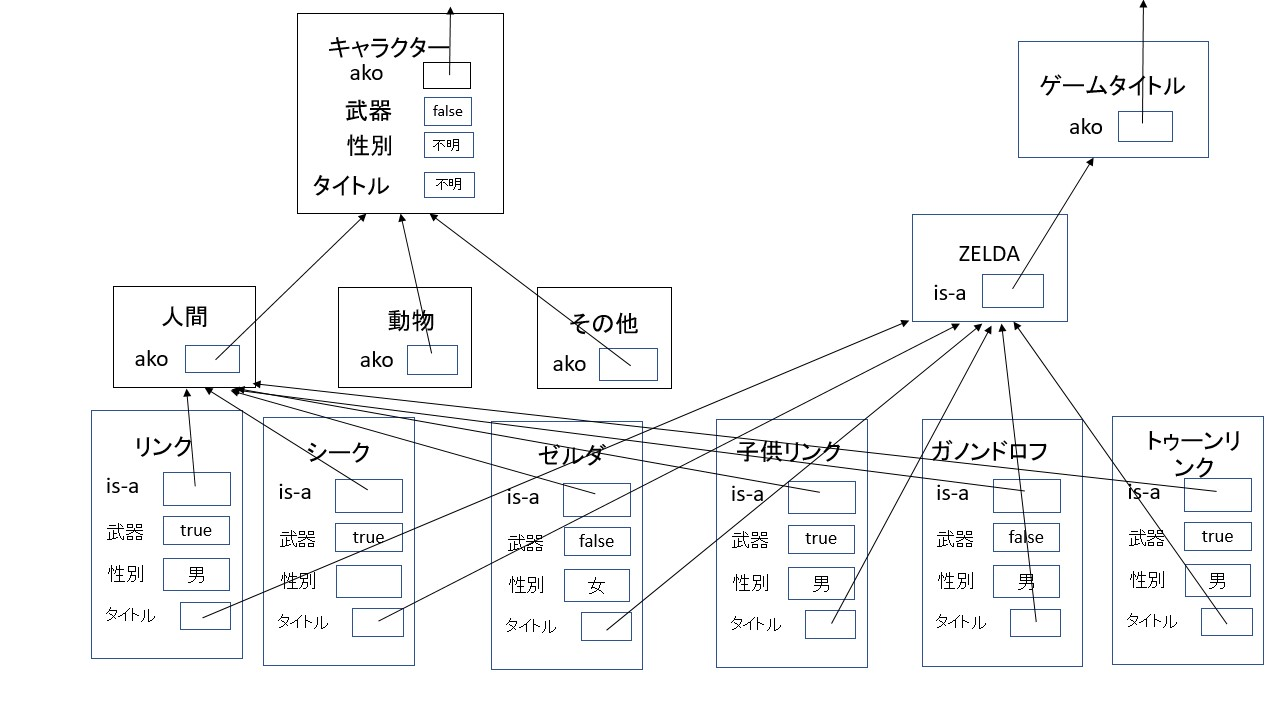
\includegraphics[width=150mm,height=80mm]{Slide1.jpg}

この図において「キャラクター」「人間」「動物」「その他」「ゲームタイトル」フレームをクラスフレーム、それ以外をインスタンスフレームとして構築している。


\subsection{実装}
上に示したフレームをMakeFrame.javaにおいて生成する.フレームの生成はExample.javaを元に実装した.なおフレームの構築
において、キャラクターのスロットにゲームタイトルのインスタンスフレームを格納する必要があったため、生成したフレームを格納しているHashMapからフレームを取り出すgetFrameメソッドをAIFrameSystem.javaに、フレームの名前を取得するgetmNameメソッドをAIFrame.javaに実装した。
\subsection{実行例}
MakeFrame.javaによってフレームを生成した.ここではreadSlotValueメソッドを用いて、生成したフレームにおいて各スロットの値が正しく格納されているかを確認した.その結果の一部を以下に示す.
\\

\begin{screen}
\begin{verbatim}
Frame:リンク
武器:true
性別:男
タイトル:ZELDA
\end{verbatim}
\end{screen}

このように生成したフレームのスロットに正しい値が格納されていることがわかる.また、ここでは『リンク』フレームに関する実行結果のみを示しているが、他のフレームに関しても同様の処理をした結果、図に示したものと同様のフレームが生成されたことを確認した.

\section{考察}
今回生成したフレームはJavaにおけるクラスの論理構造と酷似する点が多い.例えば、フレームにおけるスロットはクラスにおけるクラス・インスタンス変数に相当し、フレームのクラス・インスタンスフレームの関係はそのままクラス・インスタンスや継承に相当する.しかし、構築されるネットワークが複雑になればなるほどクラスのみを用いて実装することは困難になり、フレームやスロットの追加はフレームの方が容易になることが予想できる.今回のように小規模のネットワークではこの効力があまり実感できなかったが、自然言語の意味推論や現実世界の知識構造のように巨大なネットワークを構築する際には効力を発揮すると考える。

\section{感想}
\end{document}
